\documentclass{article}

\usepackage{graphicx}

\begin{document}

\section{Greetings}
Hello Seeking mathematicians who could better understand his work, in 1913 he began a postal partnership with the English mathematician G. H. Hardy at the University of Cambridge, England. Recognizing the extraordinary work sent to him as samples, Hardy arranged travel for Ramanujan to Cambridge. In his notes, Ramanujan had produced groundbreaking new theorems, including some that Hardy stated had "defeated him and his colleagues completely", in addition to rediscovering recently proven but highly advanced results.

\subsection{Greetings}
Hello Seeking mathematicians who could better understand his work, in 1913 he began a postal partnership with the English mathematician G. H. Hardy at the University of Cambridge, England. Recognizing the extraordinary work sent to him as samples, Hardy arranged travel for Ramanujan to Cambridge. In his notes, Ramanujan had produced groundbreaking new theorems, including some that Hardy stated had "defeated him and his colleagues completely", in addition to rediscovering recently proven but highly advanced results.

\paragraph{paraone}
Hello Seeking mathematicians who could better understand his work, in 1913 he began a postal partnership with the English mathematician G. H. Hardy at the University of Cambridge, England. Recognizing the extraordinary work sent to him as samples, Hardy arranged travel for Ramanujan to Cambridge. In his notes, Ramanujan had produced groundbreaking new theorems, including some that Hardy stated had "defeated him and his colleagues completely", in addition to rediscovering recently proven but highly advanced results.

\subparagraph{subparaone}
Hello Seeking mathematicians who could better understand his work, in 1913 he began a postal partnership with the English mathematician G. H. Hardy at the University of Cambridge, England. Recognizing the extraordinary work sent to him as samples, Hardy arranged travel for Ramanujan to Cambridge. In his notes, Ramanujan had produced groundbreaking new theorems, including some that Hardy stated had "defeated him and his colleagues completely", in addition to rediscovering recently proven but highly advanced results.

\begin{figure}
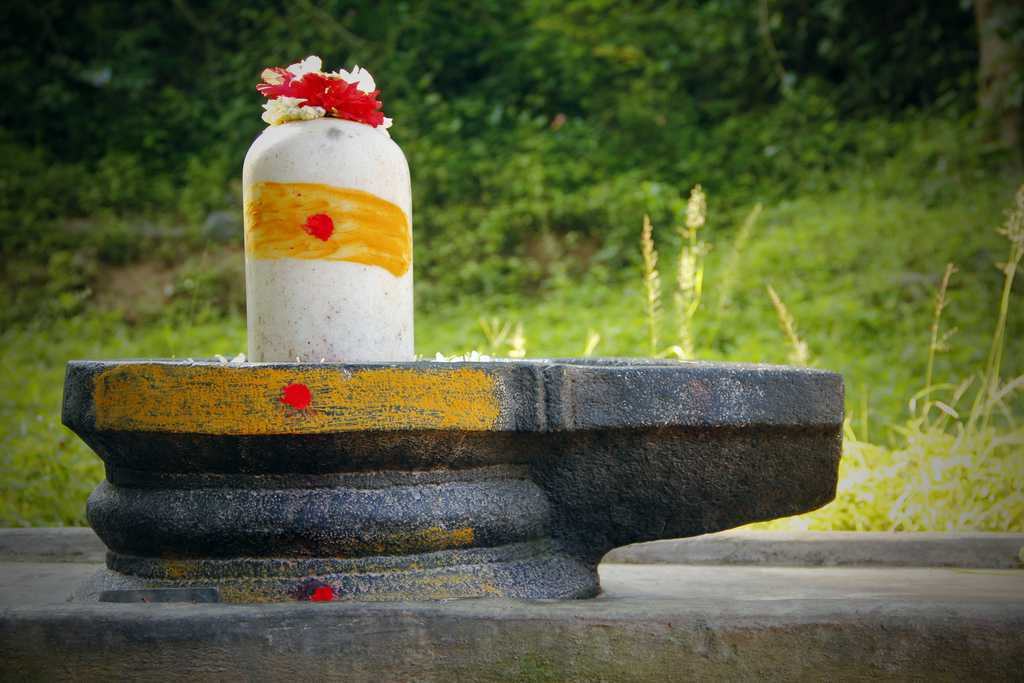
\includegraphics{shiv.jpg}
\caption{hello}
\end{figure}

\begin{tabular}{|c|c|}
\hline
abc & cde \\ \hline
fgh & ghi \\ \hline
\end{tabular}

\begin{enumerate}
\item apple
\item orange
\end{enumerate}

\section{Greetings}
Hello Seeking mathematicians who could better understand his work, in 1913 he began a postal partnership with the English mathematician G. H. Hardy at the University of Cambridge, England. Recognizing the extraordinary work sent to him as samples, Hardy arranged travel for Ramanujan to Cambridge. In his notes, Ramanujan had produced groundbreaking new theorems, including some that Hardy stated had "defeated him and his colleagues completely", in addition to rediscovering recently proven but highly advanced results.

\begin{enumerate}
\item apple
\item orange
\end{enumerate}

\begin{figure}
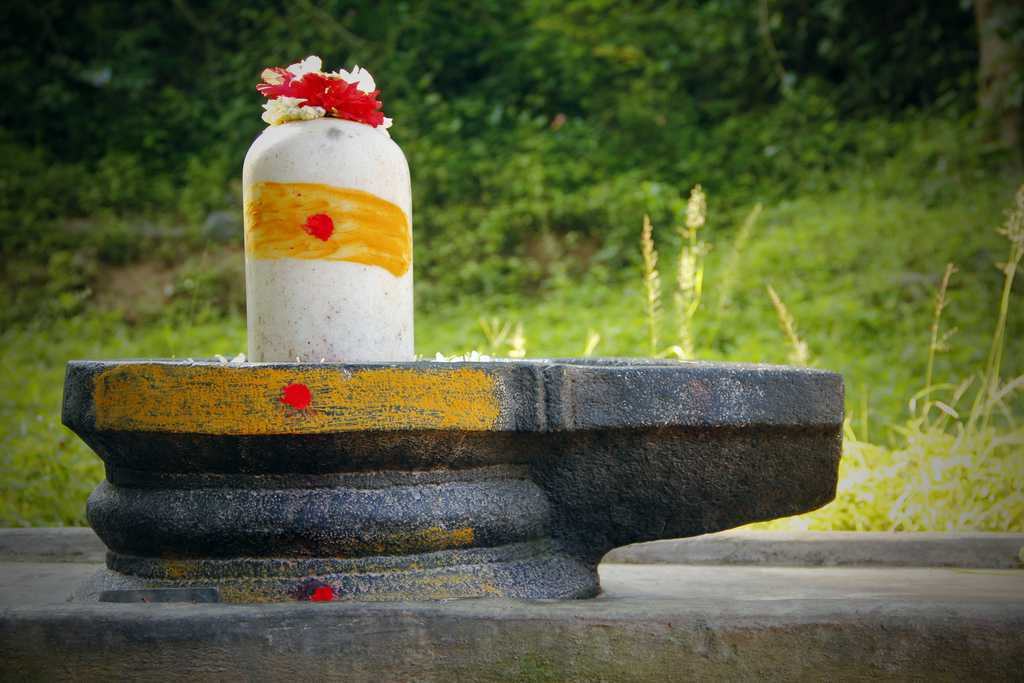
\includegraphics{shiv.jpg}
\caption{hello}
\end{figure}

\begin{figure}
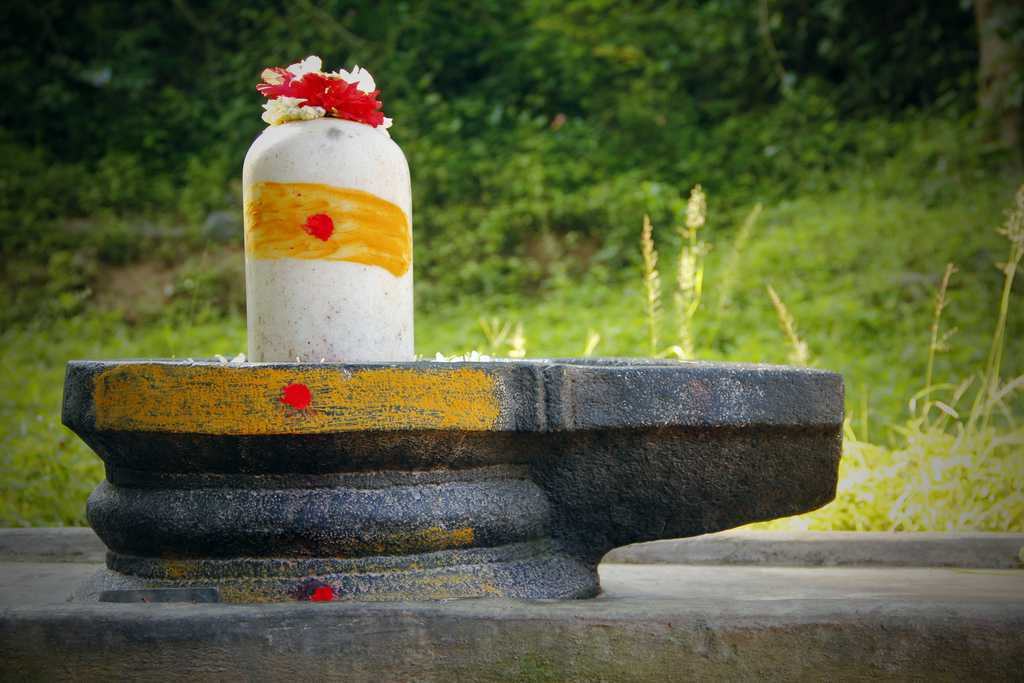
\includegraphics{shiv.jpg}
\caption{hello}
\end{figure}

\begin{tabular}{|c|c|}
\hline
abc & cde \\ \hline
fgh & ghi \\ \hline
\end{tabular}

\begin{tabular}{|c|c|}
\hline
abc & cde \\ \hline
fgh & ghi \\ \hline
\end{tabular}

\end{document}
